% (C) Marc Lijour, 2017 
% Licensed under a Creative Commons License BY-SA
% https://creativecommons.org/licenses/by-sa/2.5/ca/
% Presentation shared at the IIBS college, Mississauga, for College Campus Cash
% authored by Marc Lijour, December 2017
% 
% ======================================================================================================
%                                     Introduction to Ethereum
% ======================================================================================================
\section{Introduction to Ethereum}
\frame{
	\frametitle{Ethereum}
	%\framesubtitle{}
	\begin{columns}
	\column{0.5\textwidth}
		Ethereum is a \textbf{decentralized platform that runs smart contracts}: applications that run exactly as programmed without any possibility of downtime, censorship, fraud or third party interference.\\
		--- \url{https://ethereum.org}
	\column{0.5\textwidth}
		\begin{figure}
			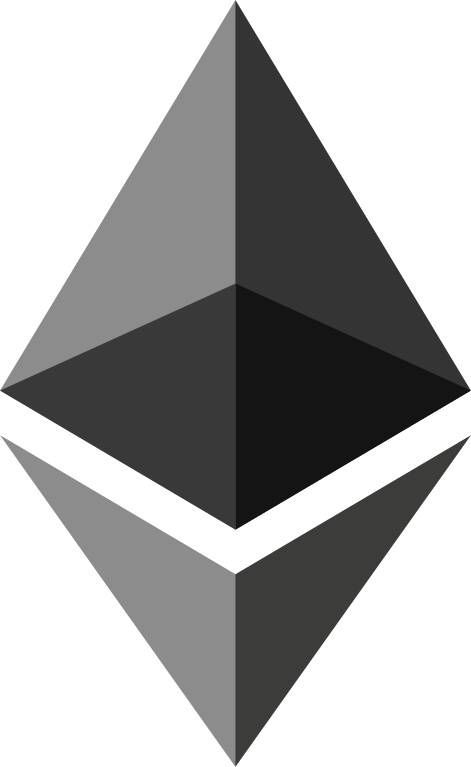
\includegraphics[height=6cm]{../pics/ethereum/471px-Ethereum_logo_2014}
		\end{figure}
	\end{columns}
}

\frame{
	\frametitle{A short history of Ethereum}
	Key Milestones:
	\begin{itemize}
		\item (late 2013) Vitalik Buterin describes Ethereum in a paper
		\pause
		\item (Summer 2014) Ethereum raises more than \$14 million in pre-sale
		\pause
		\item (July 30, 2015) Launch of Frontier, initial (beta) version of Ethereum 
		\pause
		\item (March 14, 2016) Launch of Homestead, first production release
		\pause
		\item (Spring 2016) The DAO
		\pause
		\item (July 2, 2016) ETH -- ETC split
		\pause
		\item (October 16, 2017) Launch of Metropolis (vByzantium) --version 3
		\pause
		\item (2017) ETH goes from ~\$7 to more than \$700 (100x increase)
	\end{itemize}
	\vspace{1em}
	\emph{Check the \href{https://cdn4.benzinga.com/files/images/2017/July/05/invezz-eth-history-base.jpg}{nice infographic (\cite{ethinfographic})}.}\\
	\vspace{.5em}
	Also, see the official \href{https://github.com/ethereum/wiki/wiki/White-Paper}{\emph{Ethereum White Paper}}.
}

\frame{
	\frametitle{Store of value}
	\begin{figure}
	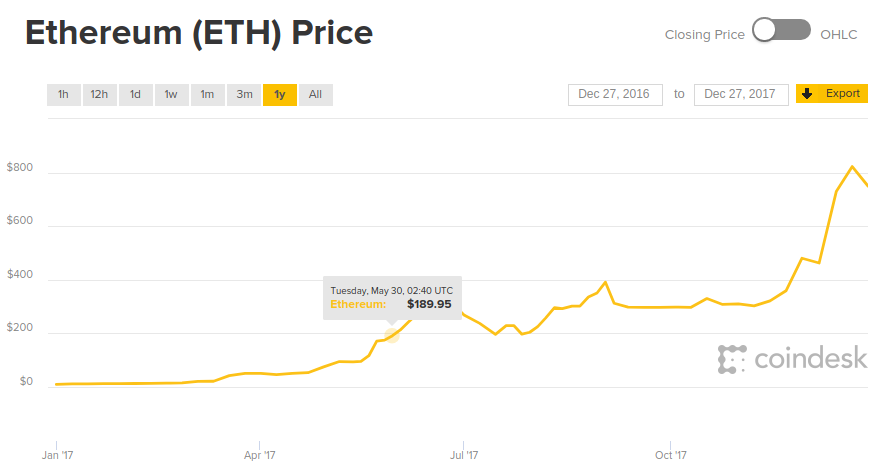
\includegraphics[height=6cm]{../pics/ethereum/ETH-price-2017}
		\caption{ETH price (\cite{coindesk:eth-price})}
		%\caption{Credit: \href{https://www.coindesk.com/ethereum-price/}{Coindesk}}
	\end{figure}
}

\frame{
	\frametitle{Decentralization}
	\begin{figure}
		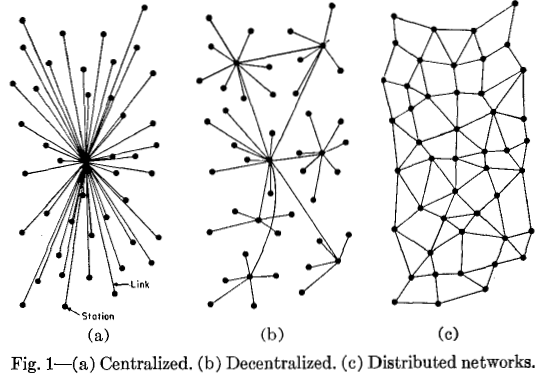
\includegraphics[height=6cm]{../pics/ethereum/networktypes}
	\end{figure}
}

\frame{
	\frametitle{Client Types}
}

\frame{
	\frametitle{Disk Space}
	\framesubtitle{With Geth \texttt{--syncmode fast} (default mode)}
	This mode initializes a $\sim$20~GB database, then turns in full node. 
	\begin{figure}
	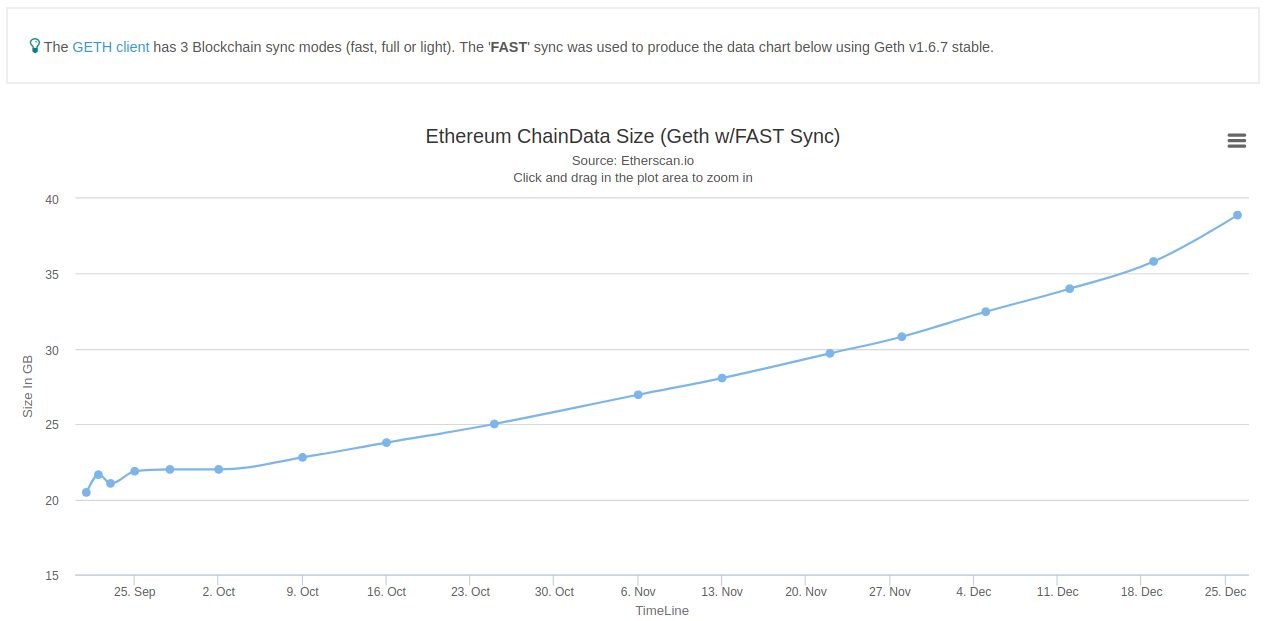
\includegraphics[height=5.5cm]{../pics/ethereum/etherscan-chaindata-2017-12-27}
		\caption{Disk space used by Geth (in fast mode) (\cite{etherscan:chaindatasize})}
	\end{figure}
}

\frame{
	\frametitle{Disk Space}
	\framesubtitle{Full Archive Ethereum node}
	\begin{figure}
	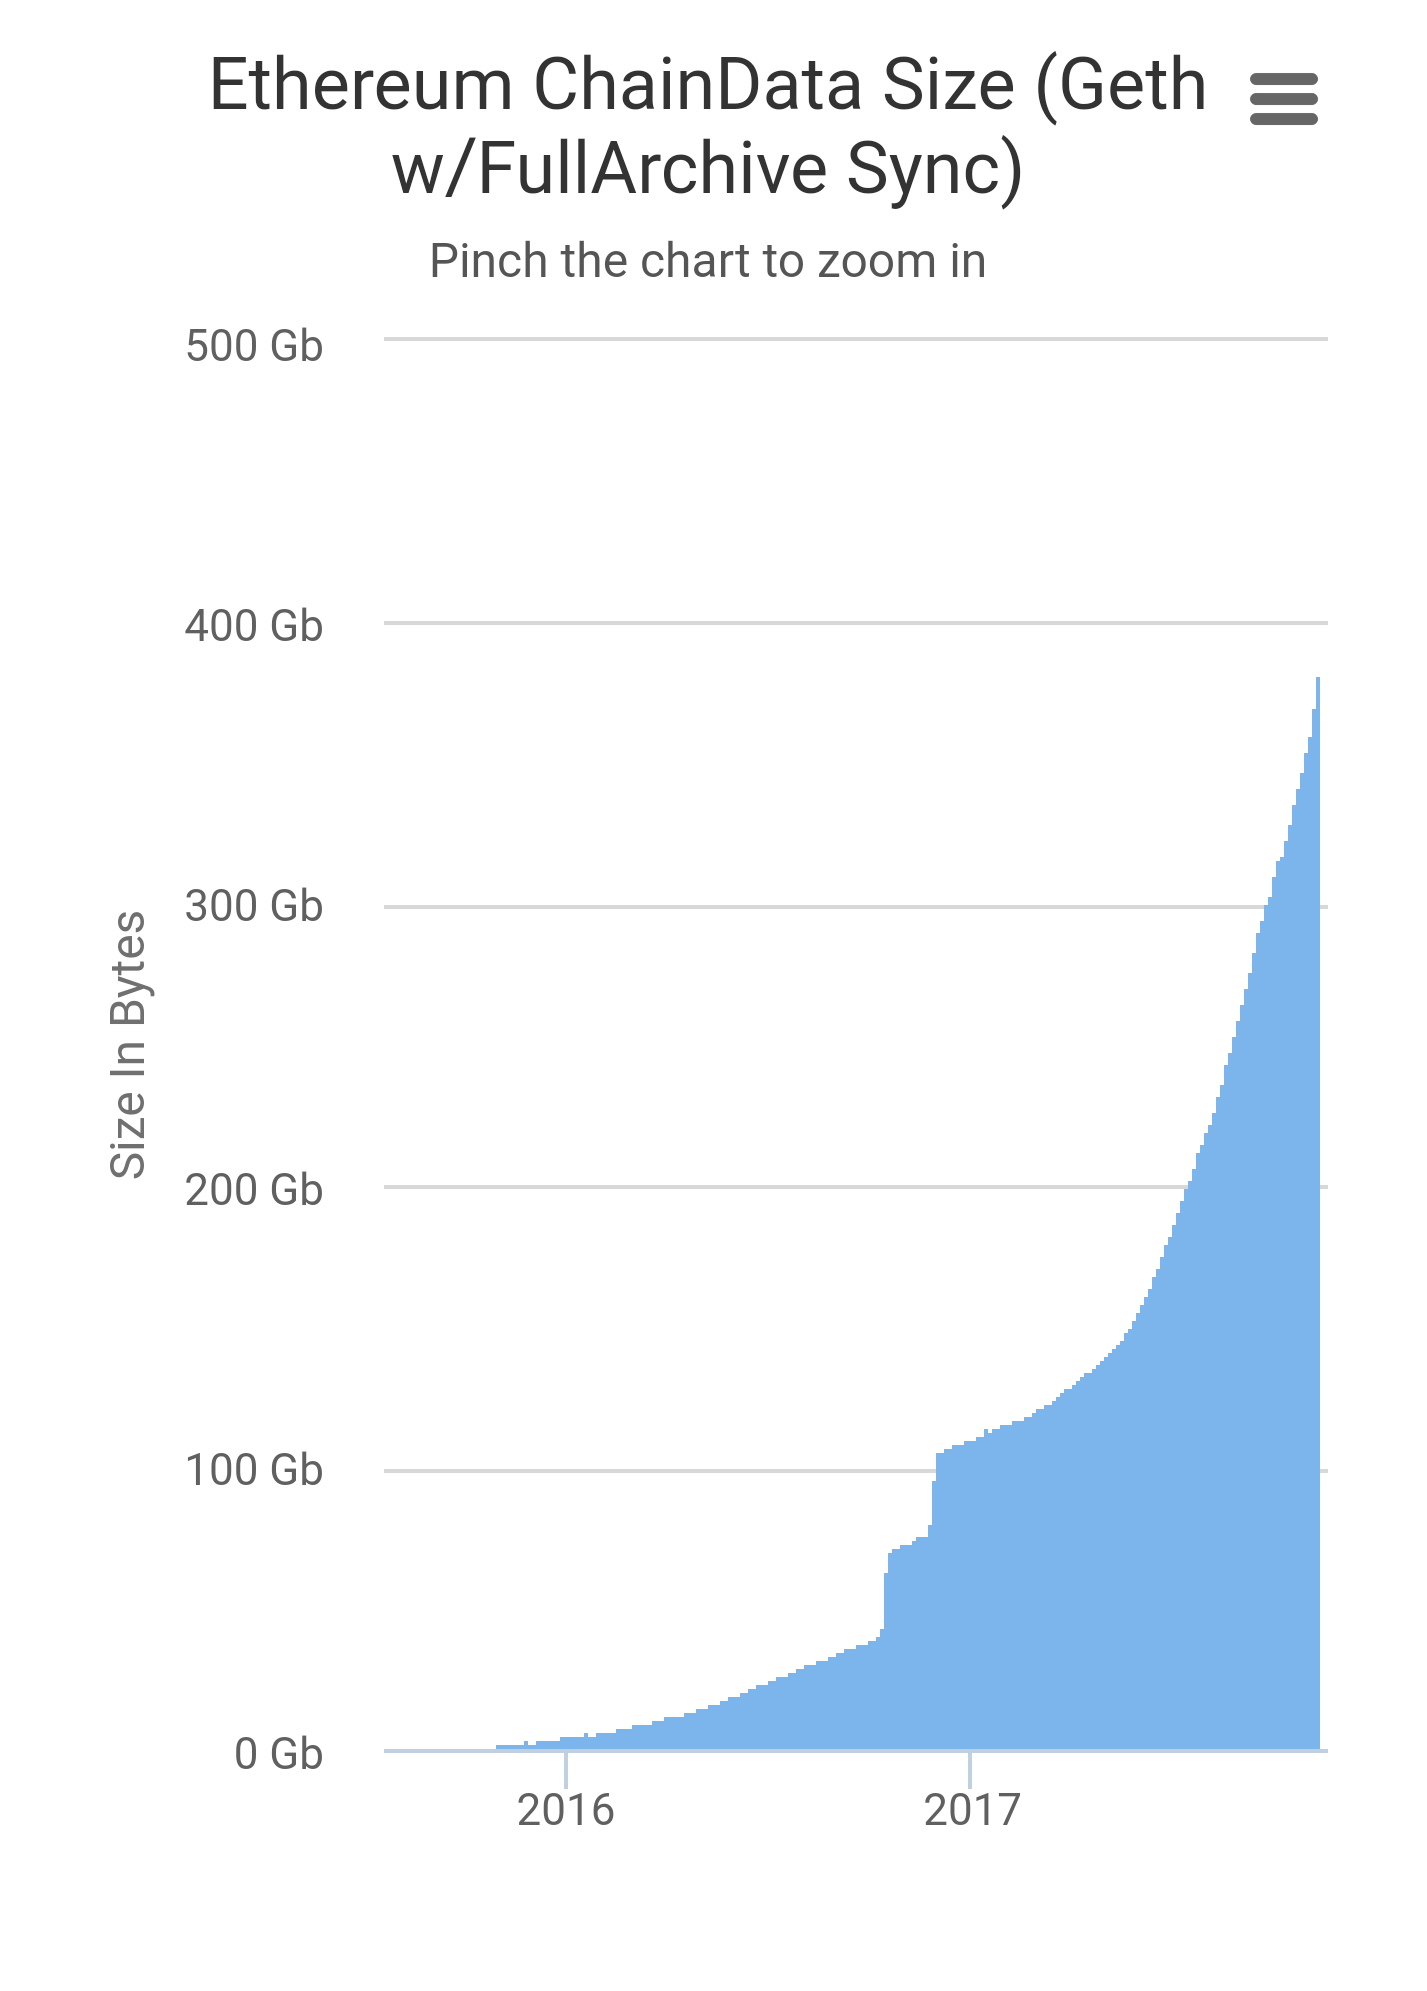
\includegraphics[height=6cm]{../pics/ethereum/geth-full-archive}
		\caption{Miners need a lot of space (\cite{reddit:chaindatasize})}
	\end{figure}
}

\frame{
	\frametitle{Disk Space}
	\framesubtitle{Ethereum vs. Bitcoin}
	\begin{figure}
	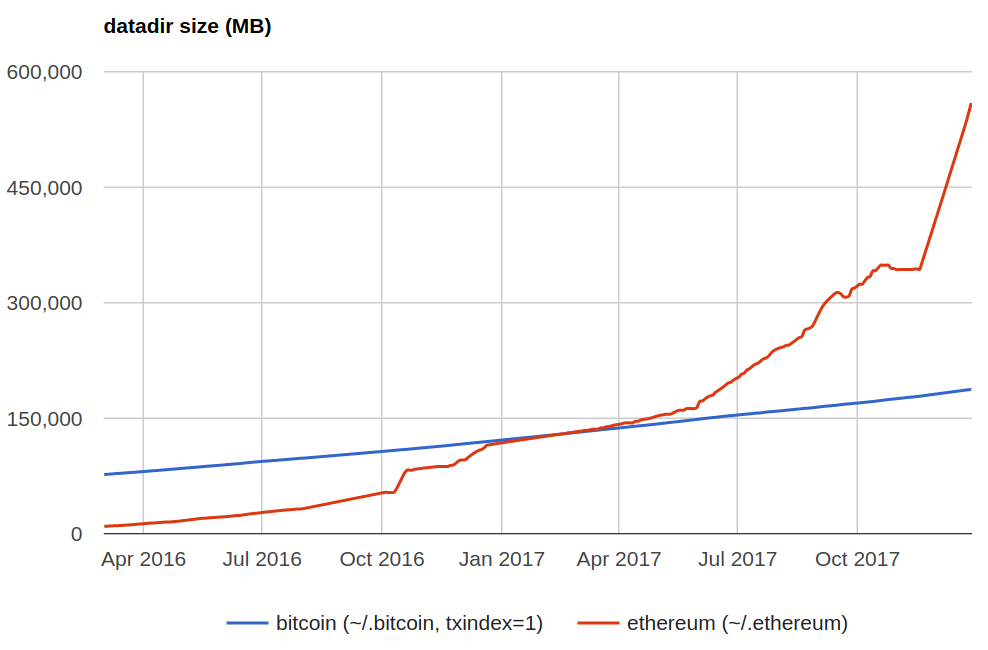
\includegraphics[height=6cm]{../pics/ethereum/daniel_net-datadir_size}
		\caption{Disk space used by Geth (\texttt{fast}) vs. Bitcoin (\cite{daniel:chaindatasize})}
	\end{figure}
}

\frame{
	\frametitle{Disk Space}
	\framesubtitle{Parity allows for continuous state trie pruning}
	In green, the configuration running as \emph{full node}.\\
	A light client can fit in $\sim$5~MB.
	\begin{figure}
	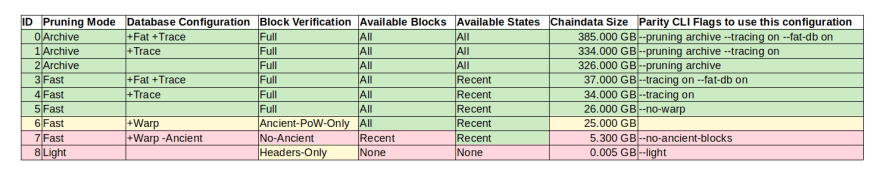
\includegraphics[width=12cm]{../pics/ethereum/afri-parity-size-2017-12}
		\caption{Disk space used by Parity (\cite{afri:chaindatasize})}
	\end{figure}
}


\frame{
	\frametitle{}
}

% ======================================================================================================
%                                     Hands-on Introduction to Smart Contracts 
% ======================================================================================================
\section{Hands-on Smart Contracts}
\frame{
	\frametitle{Install Metamask}

}

